% 2008 年重庆卷文科第 20 题：平面 α、β 相交于 l，A∈α、B∈β，AA'=3、BB'=2，
%   A'、B' 为 A、B 在 l 上的射影，二面角 α-l-β 为 2π/3。
% 来源 PDF：gaokaomath-src/普通高考/2008/2008重庆文.pdf
% SHA-256：a3f3321148dc97354de71daf028e7718ef3c3d89e634f94291448acc1f55ce08
% 原页：2008重庆文.pdf 第 2 页（A3 三栏）第 1 栏，书页码 432。
% 重绘依据：按原页斜二测画法：α 为水平面、β 为左侧斜置半平面，交线 l 为中间直线；
%   A 在 α 内右侧、A' 为其在 l 上的射影；B 在 β 内左上、B' 为其射影；AB 为实线连线段。
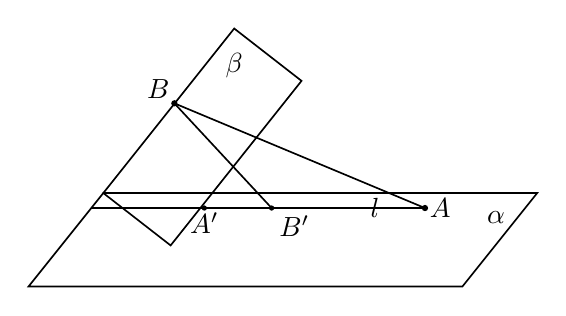
\begin{tikzpicture}[scale=0.95, semithick, every node/.style={inner sep=1.5pt}]
  % 平面 α（水平菱形）
  \draw (-1.2,-0.9) -- (4.6,-0.9) -- (5.6,0.35) -- (-0.2,0.35) -- cycle;
  \node at (5.05,0.02) {$\alpha$};
  % 平面 β（左侧斜置）
  \draw (-0.2,0.35) -- (1.55,2.55) -- (2.45,1.85) -- (0.7,-0.35) -- cycle;
  \node at (1.55,2.05) {$\beta$};
  % 交线 l
  \draw[line width=0.9pt] (-0.35,0.15) -- (3.3,0.15) node[right] {$l$};
  % 关键点
  \coordinate (Ap) at (1.15,0.15);   % A'
  \coordinate (Bp) at (2.05,0.15);   % B'
  \coordinate (A) at (4.1,0.15);
  \coordinate (B) at (0.75,1.55);
  \draw (A) -- (Ap);
  \draw (B) -- (Bp);
  \draw (A) -- (B);
  \fill (Ap) circle (1pt); \node[below] at (Ap) {$A'$};
  \fill (Bp) circle (1pt); \node[below right=1pt] at (Bp) {$B'$};
  \fill (A) circle (1.2pt); \node[right] at (A) {$A$};
  \fill (B) circle (1.2pt); \node[above left] at (B) {$B$};
\end{tikzpicture}
